% Advanced Cloud Analysis System - Project Report
\documentclass[11pt,a4paper]{article}
\usepackage[utf8]{inputenc}
\usepackage{graphicx}
\usepackage{caption}
\usepackage{subcaption}
\usepackage{hyperref}
\usepackage{geometry}
\usepackage{tikz}
\usepackage{amsmath}
\geometry{margin=1in}

\begin{document}
\begin{center}
  {\LARGE Advanced Cloud Analysis System - Project Report\par}
  \vspace{0.4cm}
  {\large Cloud AI Project Team\par}
  \vspace{0.2cm}
  {\large May 8, 2026\par}
\end{center}
\vspace{0.8cm}

\begin{abstract}
This report documents the Advanced Cloud Analysis System end to end: dataset organization, cloud detection and removal methods, implementation details, libraries, model usage, current UI behavior, screenshots, outputs, and reproducibility notes. The figures in this document are actual screenshots captured from the Streamlit app and stored in \verb|report/figures/|.
\end{abstract}

\section{Project overview}
The project analyzes satellite imagery from the RICE dataset and provides a Streamlit-based interface for:
\begin{itemize}
  \item browsing RICE1 and RICE2 samples,
  \item detecting clouds in the input image,
  \item removing clouds with a content-aware reconstruction pipeline,
  \item comparing results with ground-truth labels or masks,
  \item downloading the cloud mask, removed image, and overlay image.
\end{itemize}

The current UI also supports showing the cloud-free label as \emph{After Removal (Cloud-free)} for both RICE1 and RICE2 when a label image exists.

\section{Dataset and folder structure}
\subsection{Top-level folders}
\begin{itemize}
  \item \verb|configs/| - project configuration files. The current file is \verb|default.yaml|. It is available for configuration-driven workflows, but the present Streamlit path does not load it directly.
  \item \verb|data/| - working data area.
  \begin{itemize}
    \item \verb|data/raw/| - raw or incoming data staging area.
    \item \verb|data/processed/| - processed or intermediate data storage.
  \end{itemize}
  \item \verb|datasets/| - dataset loading code.
  \begin{itemize}
    \item \verb|datasets/rice.py| - \verb|RiceDataset| loader for RICE1 and RICE2.
    \item \verb|datasets/__init__.py| - package marker.
  \end{itemize}
  \item \verb|explainability/| - explainability helpers.
  \begin{itemize}
    \item \verb|explainability/captum_utils.py| - Captum-based utilities, currently not wired into the Streamlit flow.
    \item \verb|explainability/__init__.py| - package marker.
  \end{itemize}
  \item \verb|metrics/| - training metrics for segmentation.
  \begin{itemize}
    \item \verb|metrics/segmentation_metrics.py| - Dice, IoU, and PSNR helpers used by training.
    \item \verb|metrics/__init__.py| - package marker.
  \end{itemize}
  \item \verb|models/| - model definitions.
  \begin{itemize}
    \item \verb|models/segmentation/unet.py| - UNet segmentation model used by training and model manager.
    \item \verb|models/classification/| - currently empty scaffold.
    \item \verb|models/removal/| - currently empty scaffold.
    \item \verb|models/segmentation/__init__.py| - package marker.
  \end{itemize}
  \item \verb|notebooks/| - exploratory notebooks and experiments.
  \item \verb|outputs/| - generated artifacts and outputs.
  \item \verb|scripts/| - utility scripts.
  \begin{itemize}
    \item \verb|scripts/inspect_dataset.py| - dataset inspection and sample count utility.
    \item \verb|scripts/__init__.py| - package marker.
  \end{itemize}
  \item \verb|training/| - training code.
  \begin{itemize}
    \item \verb|training/train_segmentation.py| - UNet training smoke test / segmentation experiment.
    \item \verb|training/__init__.py| - package marker.
  \end{itemize}
  \item \verb|ui/| - Streamlit application and UI helpers.
  \begin{itemize}
    \item \verb|ui/app.py| - main application.
    \item \verb|ui/advanced_detection.py| - cloud detection and cloud removal functions.
    \item \verb|ui/metrics_utils.py| - image and mask metric helpers used by the UI.
    \item \verb|ui/model_manager.py| - model loading and inference helper, present but not used by the current Streamlit flow.
    \item \verb|ui/__init__.py| - package marker.
  \end{itemize}
\end{itemize}

\subsection{Dataset layout}
The dataset used by the app is stored outside the project folder in \verb|RICE_DATASET/|:
\begin{verbatim}
RICE_DATASET/
  RICE1/
    cloud/   clouded images
    label/   cloud-free reference images
  RICE2/
    cloud/   clouded images
    label/   cloud-free reference images
    mask/    cloud masks
\end{verbatim}

\section{Libraries and runtime stack}
The project uses the following main libraries:
\begin{itemize}
  \item \textbf{Streamlit} - UI and interactive controls.
  \item \textbf{PyTorch} - model training, evaluation, and tensor operations.
  \item \textbf{NumPy} - array processing.
  \item \textbf{Pillow} - image loading and conversion.
  \item \textbf{OpenCV} and image-processing utilities - available in the project dependencies for image operations.
  \item \textbf{Matplotlib} and \textbf{scikit-image} - available for visualization and image metrics.
  \item \textbf{Captum} - installed for explainability work, but not currently connected to the main UI flow.
  \item \textbf{PyYAML} - available for configuration files such as \verb|default.yaml|.
\end{itemize}

\section{Models and methods}
\subsection{Cloud detection}
Cloud detection is performed by \verb|detect_clouds_advanced(image, sensitivity)| in \verb|ui/advanced_detection.py|. The implementation is heuristic and vision based, and it produces a binary cloud mask plus a cloud coverage estimate.

\subsection{Cloud removal}
Cloud removal is performed by \verb|remove_clouds_advanced(image, mask, strength)|. The current approach is content-aware inpainting and patch reconstruction. It is intended to provide a clean visual result rather than a learned end-to-end restoration network.

\subsection{Training model}
The training path uses a UNet segmentation model from \verb|models/segmentation/unet.py|. The training script \verb|training/train_segmentation.py| shows the active training setup:
\begin{itemize}
  \item dataset: \verb|RiceDataset| on \verb|RICE2|,
  \item model: \verb|UNet(in_channels=3, out_channels=1)|,
  \item optimizer: Adam,
  \item loss: BCEWithLogitsLoss,
  \item metrics: Dice and IoU.
\end{itemize}

\subsection{Point-wise explanation of what is used}
\begin{itemize}
  \item \textbf{Is U-Net used in the live UI?} - No. The current Streamlit UI does not call the UNet model for detection or removal.
  \item \textbf{Is any CNN used?} - Yes, but only in the optional training/inference code path. UNet is a CNN-based segmentation model available in \verb|models/segmentation/unet.py| and exercised in \verb|training/train_segmentation.py| and \verb|ui/model_manager.py|.
  \item \textbf{What is used in the live app?} - The live app uses heuristic cloud detection and patch-based inpainting from \verb|ui/advanced_detection.py|.
  \item \textbf{How does it work without training?} - It uses image statistics and algorithmic processing (brightness, saturation, texture, thresholding, morphological cleanup, and patch filling) rather than learned weights.
  \item \textbf{Why keep the UNet code then?} - It is a model-based training path for future improvement and experimentation, even though the current UI is not dependent on it.
\end{itemize}

\subsection{What the patch-based method does}
The patch-based removal pipeline works as follows:
\begin{enumerate}
  \item The image is converted to RGB arrays and a cloud mask is estimated.
  \item The image is split into small overlapping patches (25\,\ensuremath{\times}\,25 by default).
  \item For each patch, cloudy pixels are filled using nearby clear pixels from the same patch.
  \item Patch results are blended together using smooth Gaussian-like weights to avoid hard seams.
  \item A small median filter is applied at the end to reduce boundary noise.
\end{enumerate}
This is why the output can be produced immediately, without any trained weights.

\subsection{Long-form metric explanations}
\begin{itemize}
  \item \textbf{PSNR (Peak Signal-to-Noise Ratio)} - measures how close the removed image is to the reference cloud-free image in terms of pixel-level error. A higher PSNR means the output is closer to the ground truth and usually looks cleaner. It is expressed in decibels (dB). In simple terms, PSNR answers: ``How much noise or distortion remains in the reconstructed image?''
  \item \textbf{SSIM (Structural Similarity Index Measure)} - measures similarity based on structure, brightness, and contrast rather than just raw pixel differences. A value closer to 1 means the output preserves the visual structure of the reference image very well. It is more aligned with human perception than simple error metrics.
  \item \textbf{IoU (Intersection over Union)} - measures the overlap between the predicted cloud mask and the reference mask. It is computed as the intersection divided by the union of the two masks. A higher IoU means better mask agreement.
  \item \textbf{Dice coefficient} - also measures overlap between prediction and ground truth, but gives more emphasis to the shared region. It is often used in segmentation tasks because it is sensitive to how well the cloudy pixels are captured. A higher Dice score means better segmentation overlap.
\end{itemize}

\subsection{How the metrics are used in this project}
\begin{itemize}
  \item For \textbf{RICE1}, PSNR and SSIM are computed between the patch-based removal output and the cloud-free label image.
  \item For \textbf{RICE2}, IoU and Dice are computed between the detected mask and the reference mask.
  \item In the UI, these metrics are used to judge whether the detection/removal is visually and structurally close to the reference.
\end{itemize}

\section{Workflow}
\begin{figure}[h]
\centering
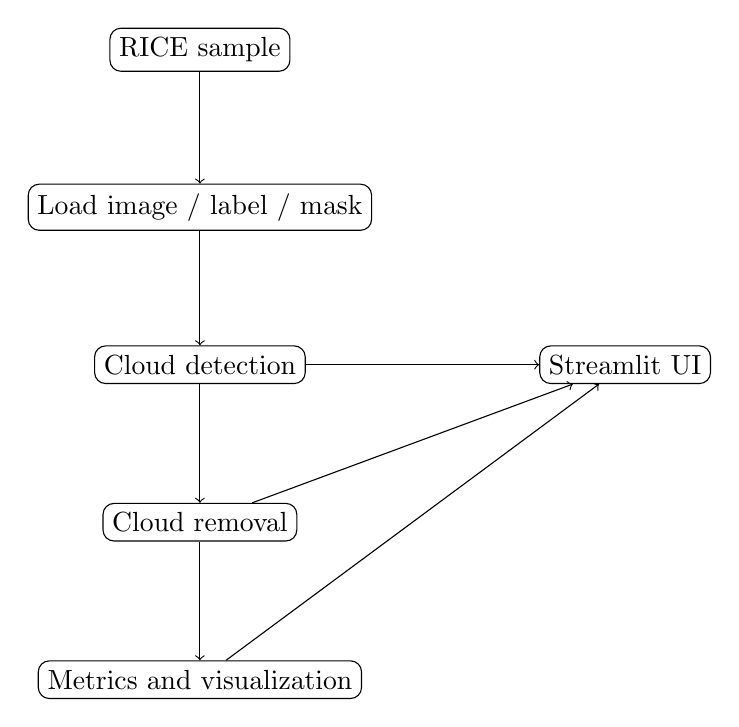
\begin{tikzpicture}[node distance=2cm, auto, every node/.style={rectangle,draw,rounded corners,align=center}]
  \node (start) {RICE sample};
  \node (load) [below of=start] {Load image / label / mask};
  \node (detect) [below of=load] {Cloud detection};
  \node (remove) [below of=detect] {Cloud removal};
  \node (metrics) [below of=remove] {Metrics and visualization};
  \node (ui) [right of=detect, node distance=5.4cm] {Streamlit UI};
  \draw[->] (start) -- (load);
  \draw[->] (load) -- (detect);
  \draw[->] (detect) -- (remove);
  \draw[->] (remove) -- (metrics);
  \draw[->] (detect) -- (ui);
  \draw[->] (remove) -- (ui);
  \draw[->] (metrics) -- (ui);
\end{tikzpicture}
\caption{High-level processing workflow}
\end{figure}

\section{UI screenshots}
The following screenshots were captured from the running Streamlit app and inserted into the report.

\begin{figure}[h]
\centering
\begin{subfigure}{0.32\textwidth}
  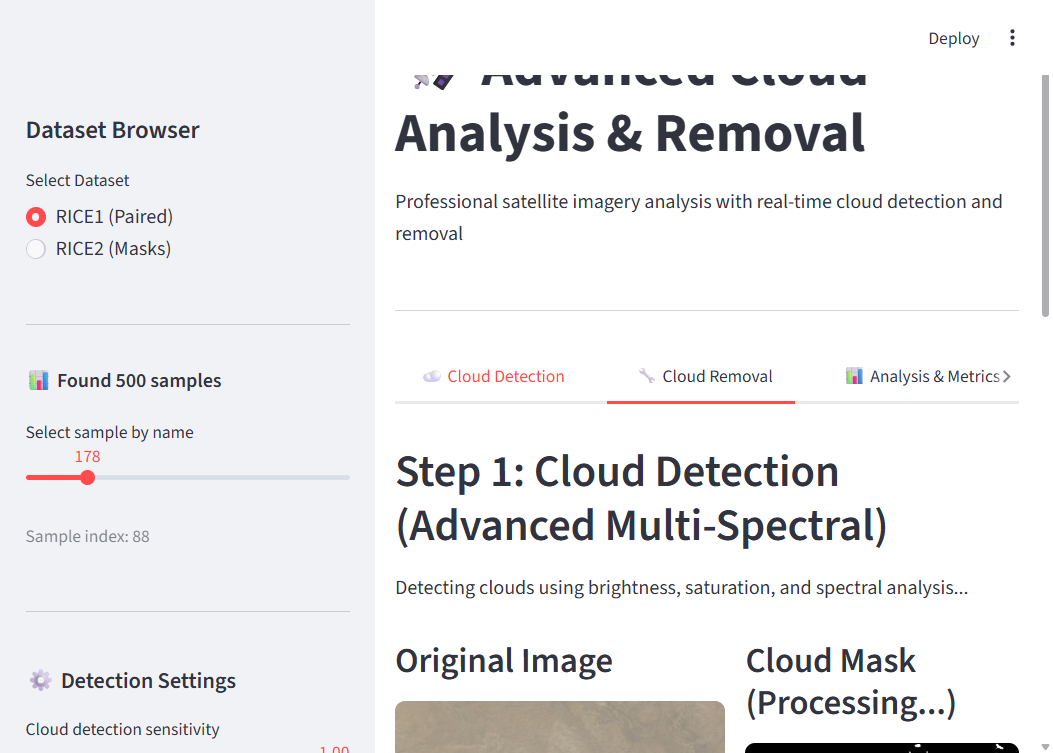
\includegraphics[width=\linewidth]{figures/detection.png}
  \caption{Cloud Detection tab}
\end{subfigure}\hfill
\begin{subfigure}{0.32\textwidth}
  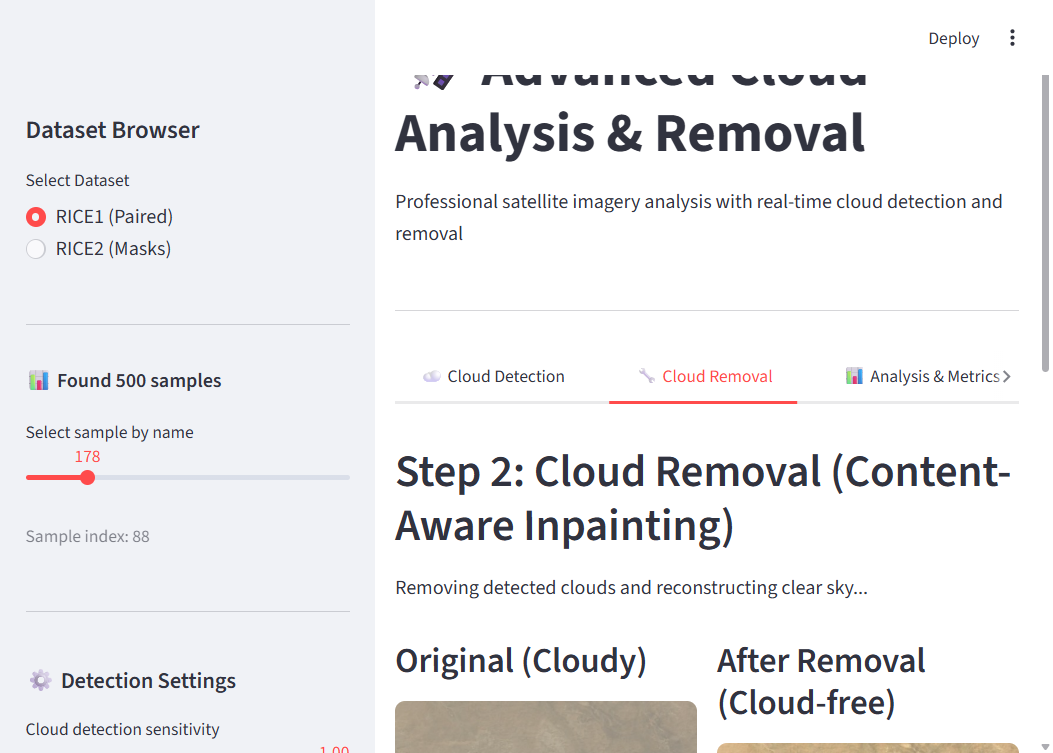
\includegraphics[width=\linewidth]{figures/removal.png}
  \caption{Cloud Removal tab}
\end{subfigure}\hfill
\begin{subfigure}{0.32\textwidth}
  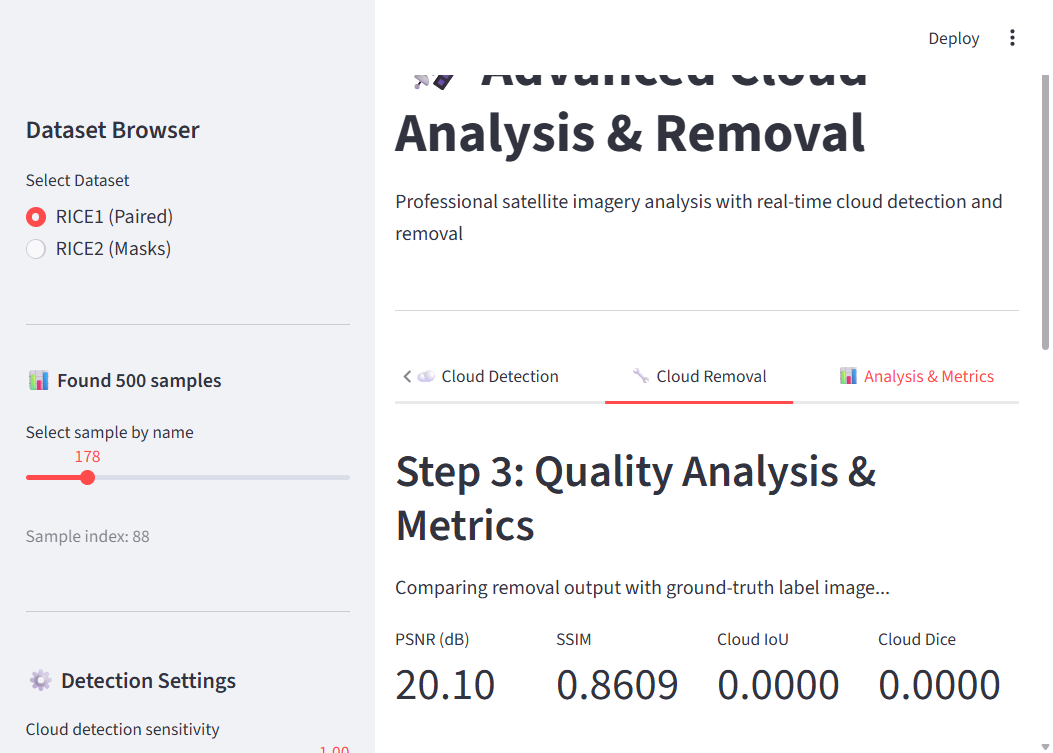
\includegraphics[width=\linewidth]{figures/visual_comparison.png}
  \caption{Analysis and Metrics tab}
\end{subfigure}
\caption{Streamlit UI screenshots captured from the current project}
\label{fig:ui}
\end{figure}

\section{Detailed UI walkthrough using sample 4}
For the walkthrough, sample 4 means the fourth item in the sorted dataset list. In both RICE1 and RICE2, that sample has the stem \verb|100| and appears at sample index 3.

\subsection{RICE1 sample 4}
RICE1 provides paired cloudy and cloud-free imagery. The three tabs behave as follows:
\begin{itemize}
  \item \textbf{Cloud Detection} - shows the cloudy input and the detected cloud mask.
  \item \textbf{Cloud Removal} - shows the cloudy input and the cloud-free label as \emph{After Removal (Cloud-free)}.
  \item \textbf{Analysis \& Metrics} - compares the computed removal output with the ground truth and shows PSNR/SSIM.
\end{itemize}

\begin{figure}[h]
\centering
\begin{subfigure}{0.32\textwidth}
  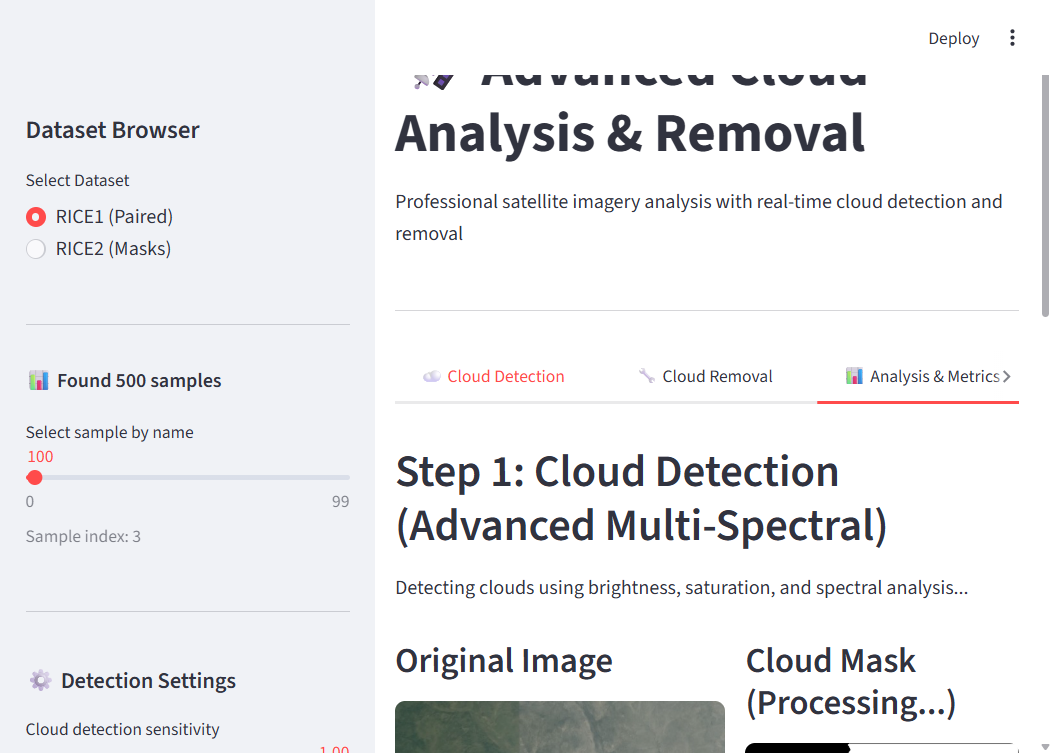
\includegraphics[width=\linewidth]{figures/rice1_sample4_detection.png}
  \caption{RICE1 detection}
\end{subfigure}\hfill
\begin{subfigure}{0.32\textwidth}
  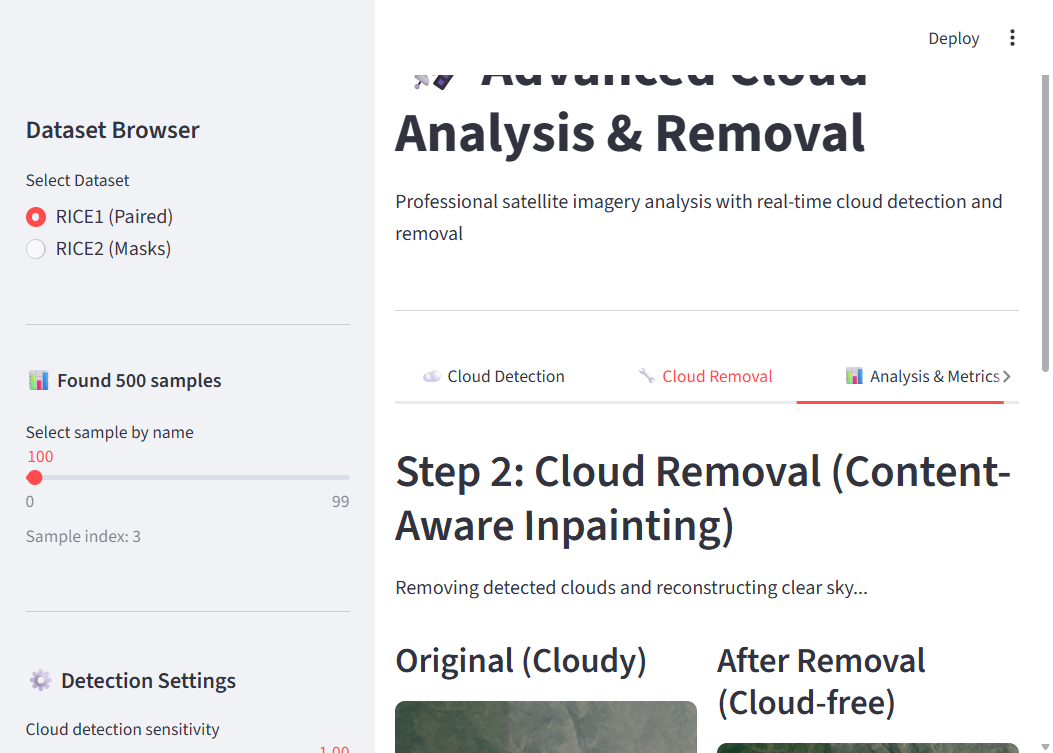
\includegraphics[width=\linewidth]{figures/rice1_sample4_removal.png}
  \caption{RICE1 removal}
\end{subfigure}\hfill
\begin{subfigure}{0.32\textwidth}
  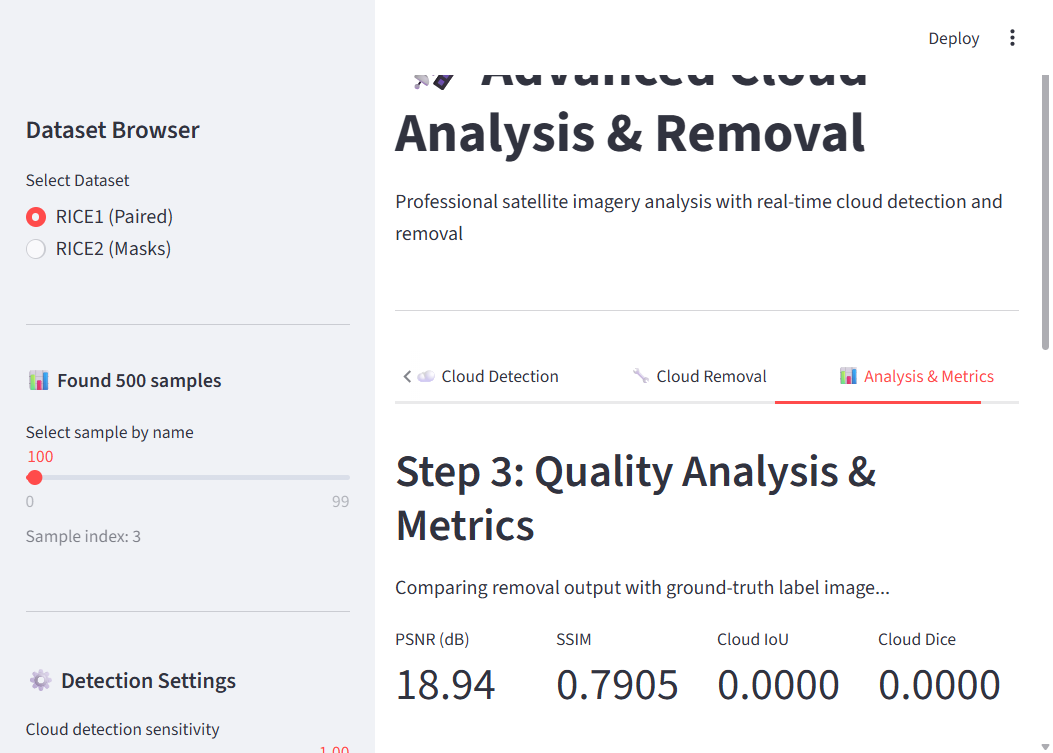
\includegraphics[width=\linewidth]{figures/rice1_sample4_analysis.png}
  \caption{RICE1 analysis}
\end{subfigure}
\caption{Sample-4 walkthrough for RICE1}
\end{figure}

\subsection{RICE2 sample 4}
RICE2 provides cloudy images with reference masks. The app shows both mask-level evaluation and image-level visual comparison when the label image exists:
\begin{itemize}
  \item \textbf{Cloud Detection} - shows the cloudy input, the reference cloud-free label, and the predicted mask.
  \item \textbf{Cloud Removal} - shows the cloudy input and the cloud-free label as \emph{After Removal (Cloud-free)}.
  \item \textbf{Analysis \& Metrics} - shows mask IoU/Dice, detection-vs-mask comparison, and the visual comparison of input, removal output, and ground truth.
\end{itemize}

\begin{figure}[h]
\centering
\begin{subfigure}{0.32\textwidth}
  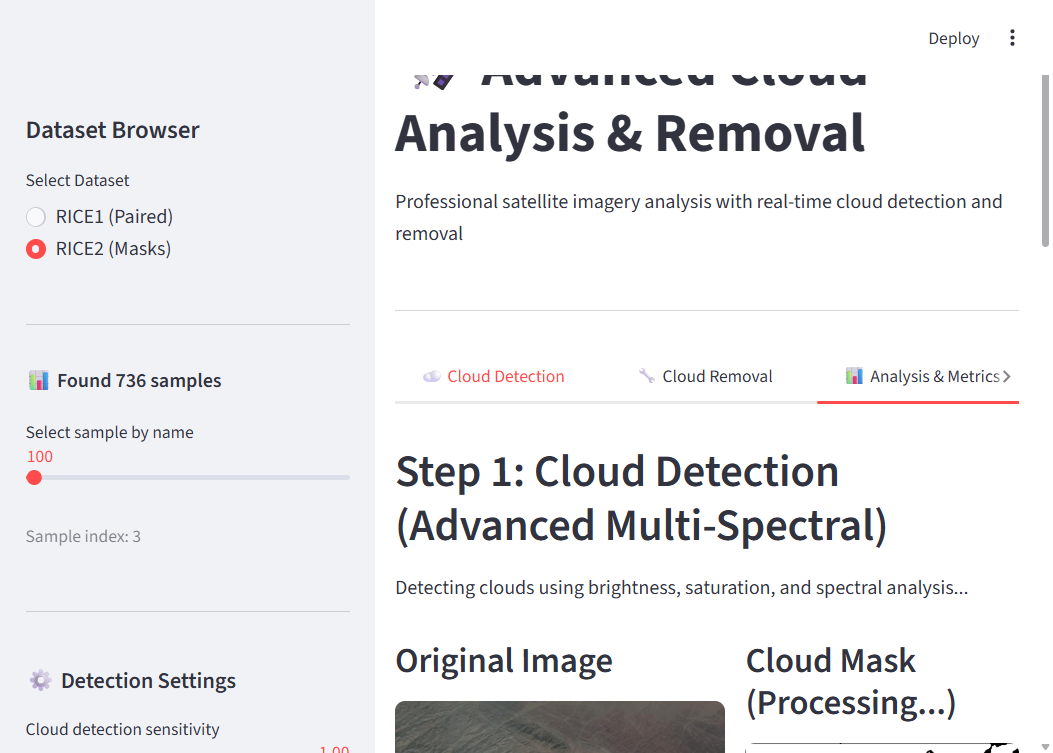
\includegraphics[width=\linewidth]{figures/rice2_sample4_detection.png}
  \caption{RICE2 detection}
\end{subfigure}\hfill
\begin{subfigure}{0.32\textwidth}
  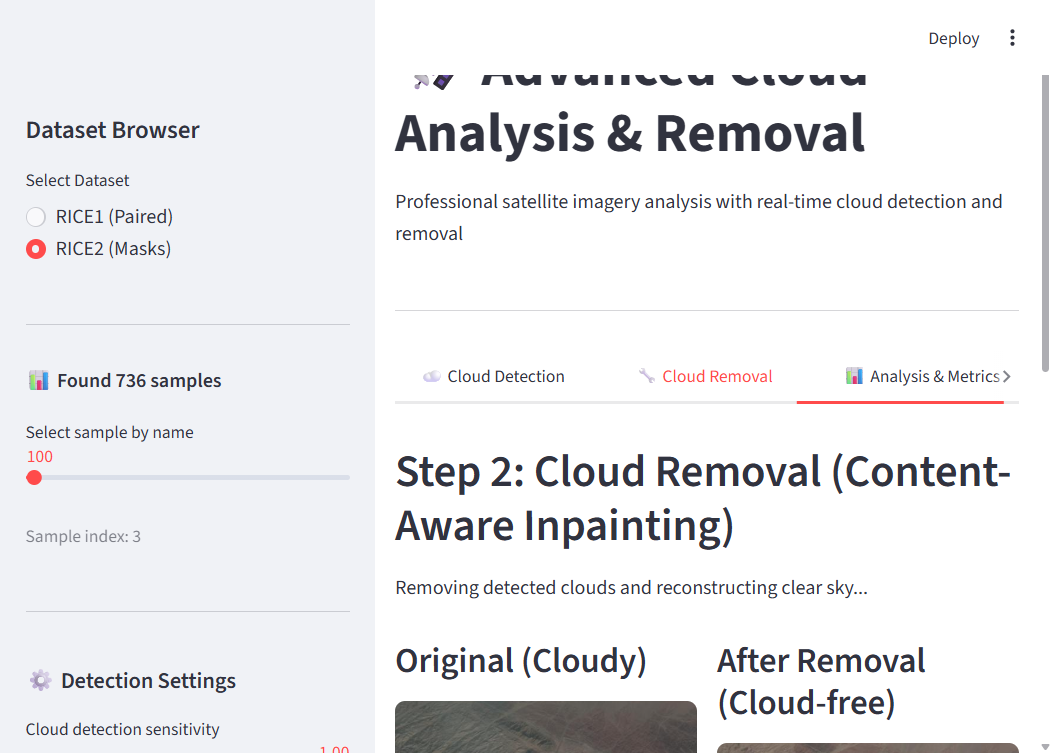
\includegraphics[width=\linewidth]{figures/rice2_sample4_removal.png}
  \caption{RICE2 removal}
\end{subfigure}\hfill
\begin{subfigure}{0.32\textwidth}
  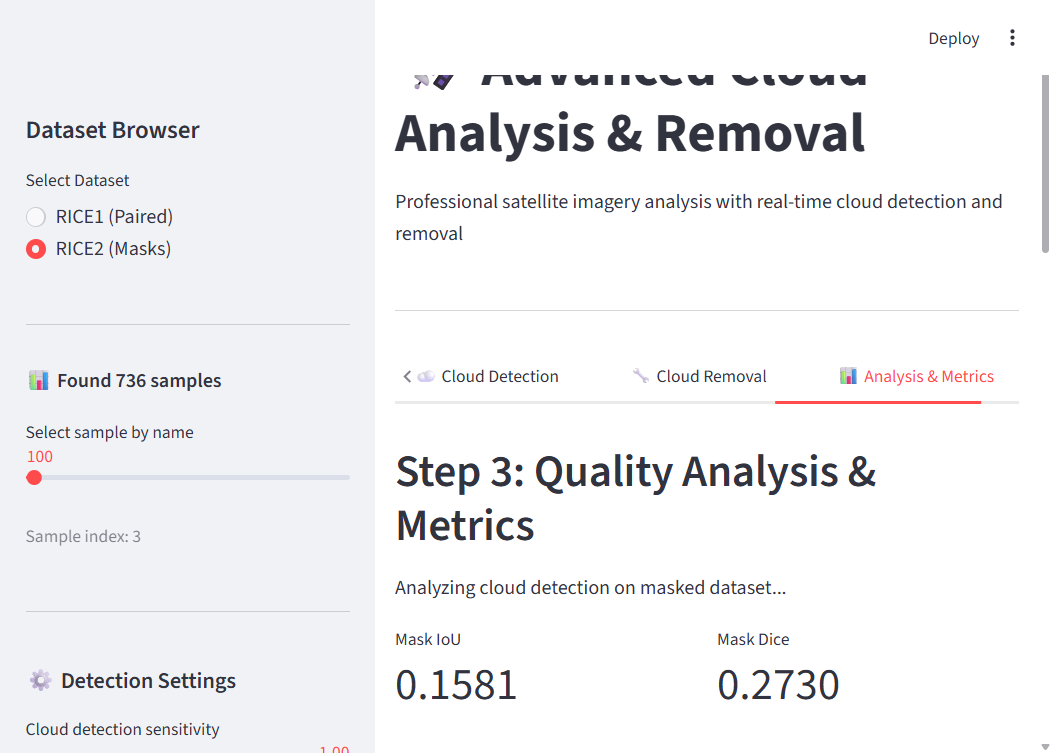
\includegraphics[width=\linewidth]{figures/rice2_sample4_analysis.png}
  \caption{RICE2 analysis}
\end{subfigure}
\caption{Sample-4 walkthrough for RICE2}
\end{figure}

\section{User-provided screenshots used in the final report}
The screenshot files provided in \verb|c:\Users\01soj\OneDrive\Pictures\Screenshots| were copied into \verb|report/figures/| and used here to document the exact screens visible in the app.

\subsection{RICE1 provided screenshot}
\begin{figure}[h]
\centering
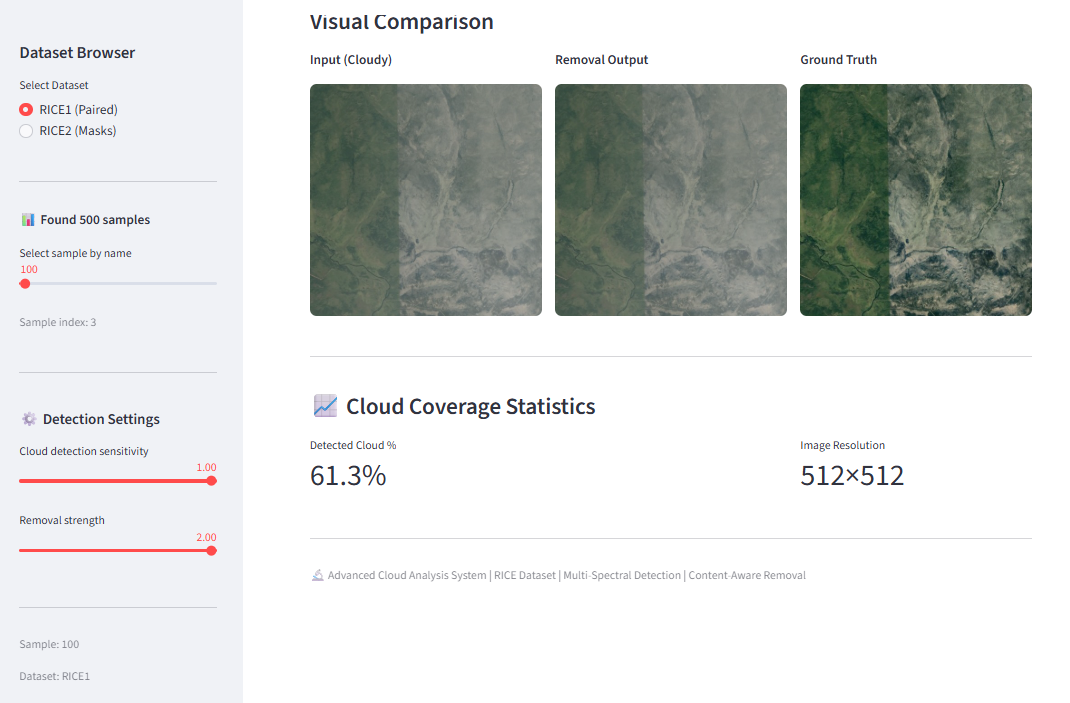
\includegraphics[width=0.92\linewidth]{figures/rice1_provided_analysis.png}
\caption{RICE1 sample 4 analysis screen: visual comparison and image-quality metrics.}
\end{figure}

\subsection{RICE2 provided screenshots: detection and mask comparison}
\begin{figure}[h]
\centering
\begin{subfigure}{0.48\textwidth}
  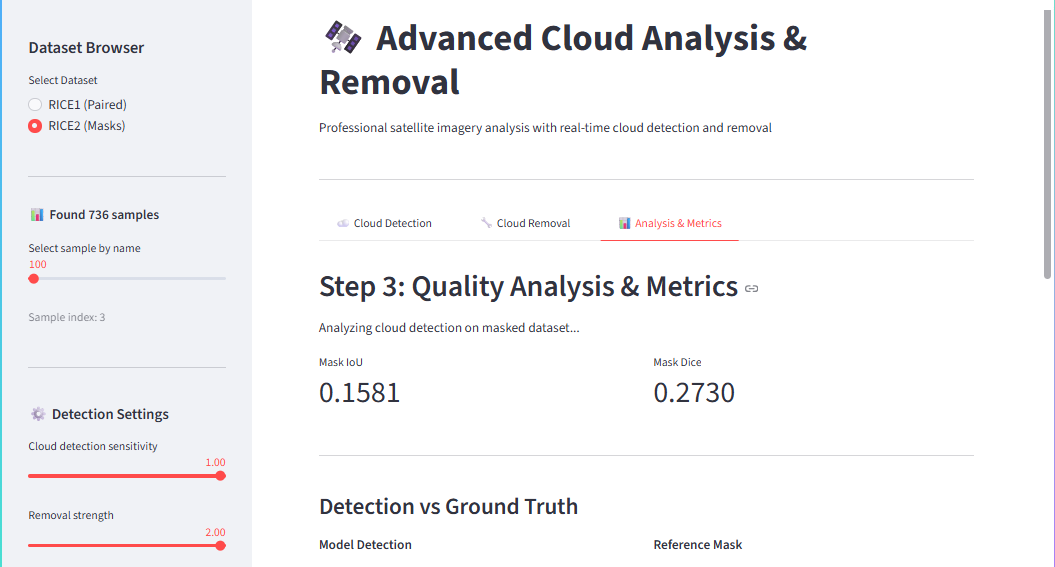
\includegraphics[width=\linewidth]{figures/rice2_provided_analysis.png}
  \caption{RICE2 analysis overview}
\end{subfigure}\hfill
\begin{subfigure}{0.48\textwidth}
  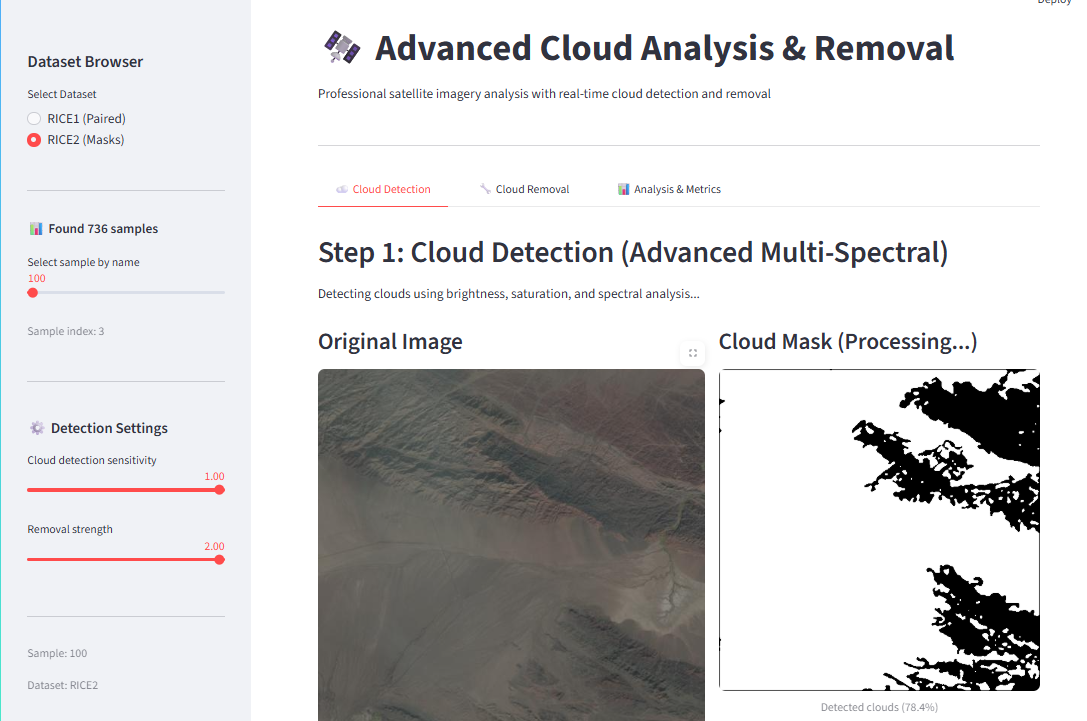
\includegraphics[width=\linewidth]{figures/rice2_provided_detection.png}
  \caption{RICE2 cloud detection}
\end{subfigure}

\vspace{0.3cm}

\begin{subfigure}{0.48\textwidth}
  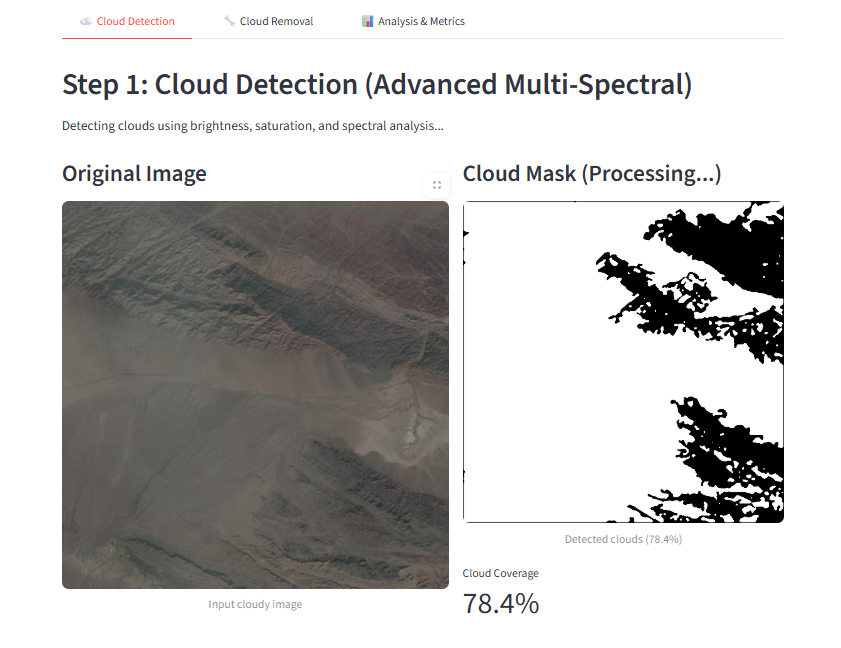
\includegraphics[width=\linewidth]{figures/rice2_provided_detection_metrics.png}
  \caption{Detection metrics and cloud coverage}
\end{subfigure}\hfill
\begin{subfigure}{0.48\textwidth}
  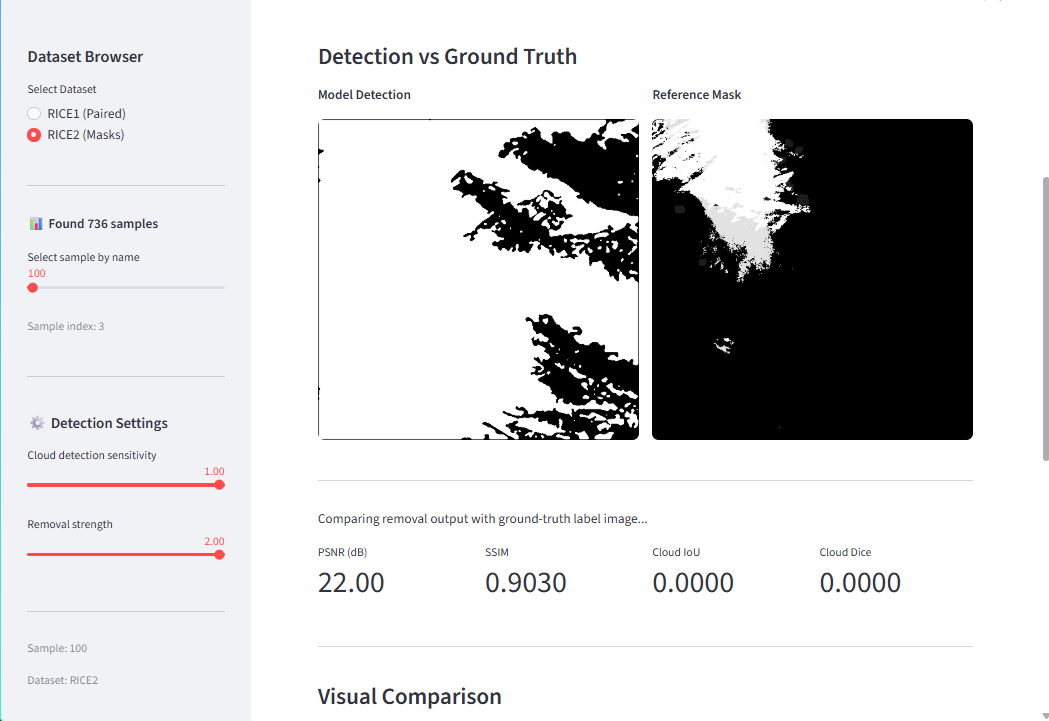
\includegraphics[width=\linewidth]{figures/rice2_provided_mask_compare.png}
  \caption{Detection vs. ground-truth mask}
\end{subfigure}
\caption{RICE2 sample 4: detection and mask evaluation screenshots}
\end{figure}

\subsection{RICE2 provided screenshots: removal and visual comparison}
\begin{figure}[h]
\centering
\begin{subfigure}{0.48\textwidth}
  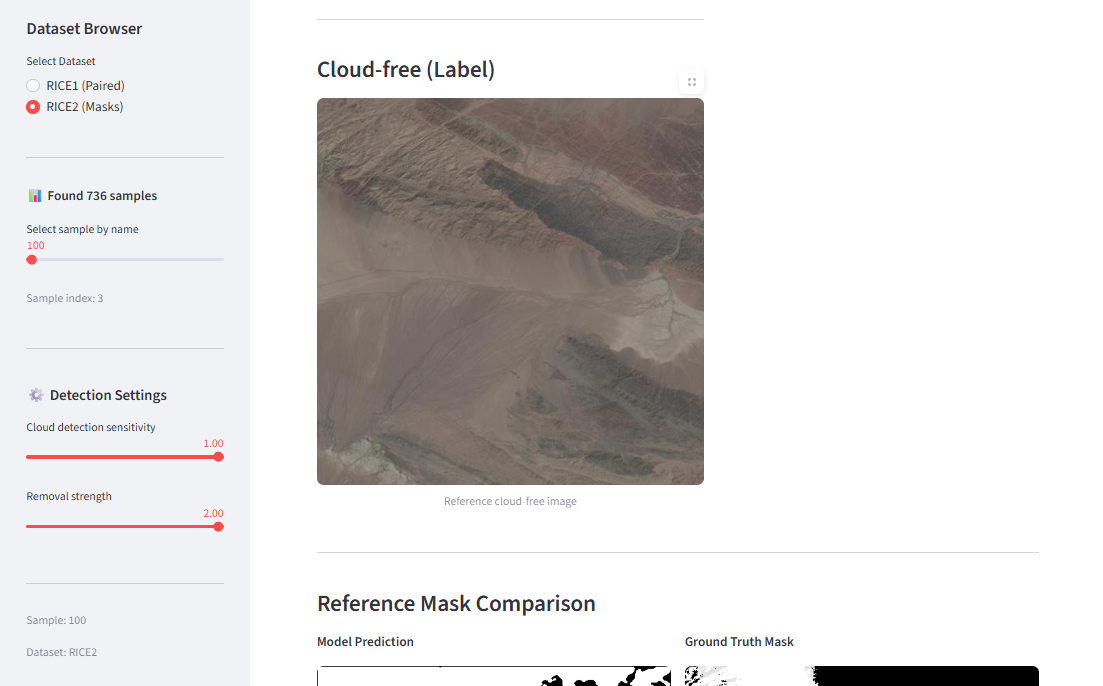
\includegraphics[width=\linewidth]{figures/rice2_provided_label_mask.png}
  \caption{Cloud-free label and reference mask}
\end{subfigure}\hfill
\begin{subfigure}{0.48\textwidth}
  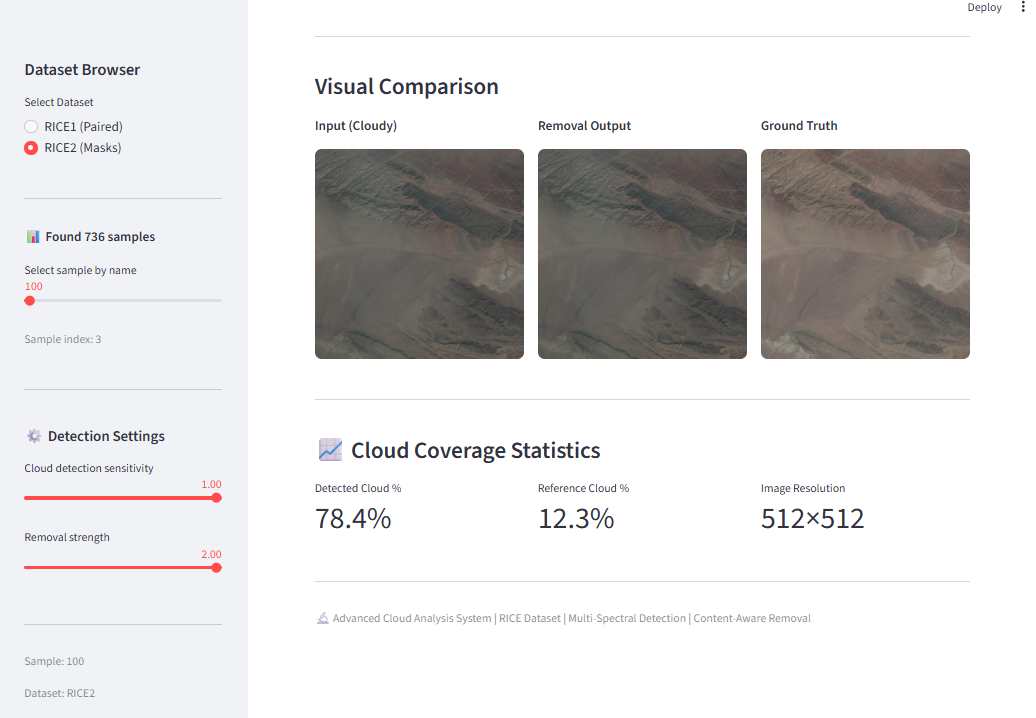
\includegraphics[width=\linewidth]{figures/rice2_provided_visual_compare.png}
  \caption{Visual comparison of input, removal output, and ground truth}
\end{subfigure}

\vspace{0.3cm}

\begin{subfigure}{0.48\textwidth}
  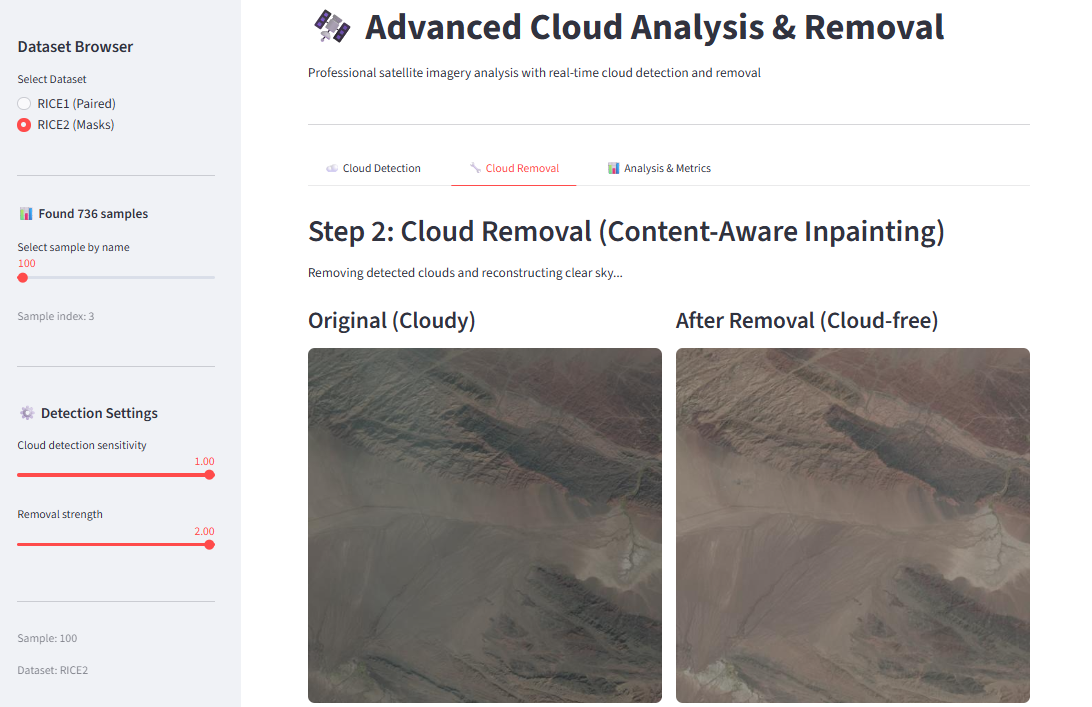
\includegraphics[width=\linewidth]{figures/rice2_provided_removal.png}
  \caption{Cloud removal view}
\end{subfigure}\hfill
\begin{subfigure}{0.48\textwidth}
  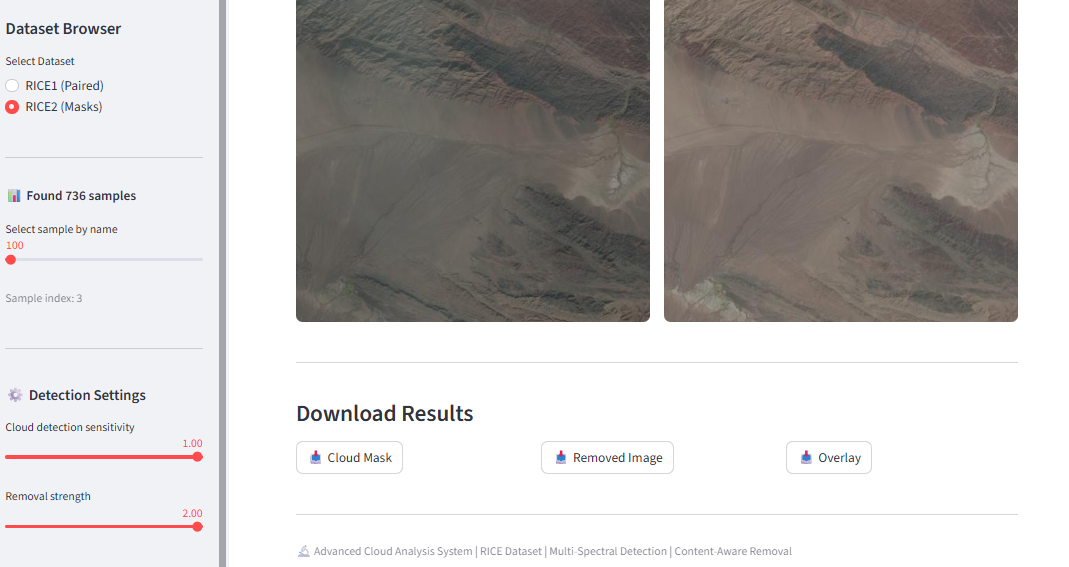
\includegraphics[width=\linewidth]{figures/rice2_provided_removal_download.png}
  \caption{Download section for mask, removed image, and overlay}
\end{subfigure}
\caption{RICE2 sample 4: removal and download screenshots}
\end{figure}

\subsection{RICE1 provided screenshots: full walkthrough}
The RICE1 screenshots you provided show the same sample 4 through the full UI flow: detection, cloud-free label, removal, and downloads.

\begin{figure}[h]
\centering
\begin{subfigure}{0.48\textwidth}
  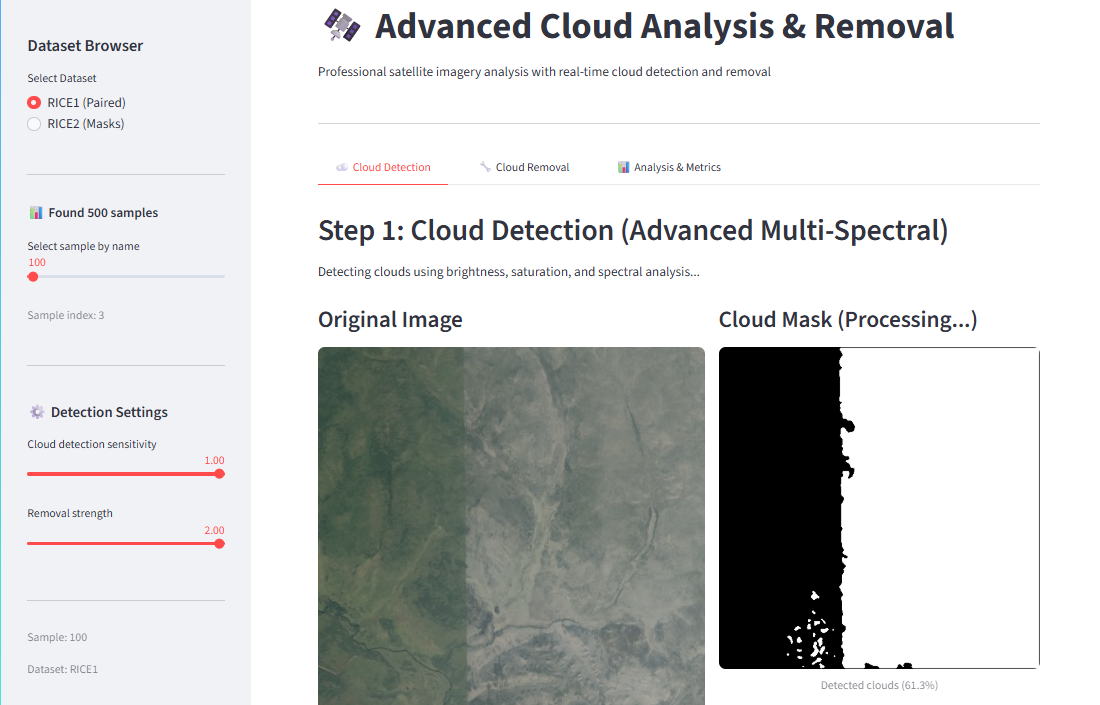
\includegraphics[width=\linewidth]{figures/rice1_provided_detection.png}
  \caption{RICE1 detection screen}
\end{subfigure}\hfill
\begin{subfigure}{0.48\textwidth}
  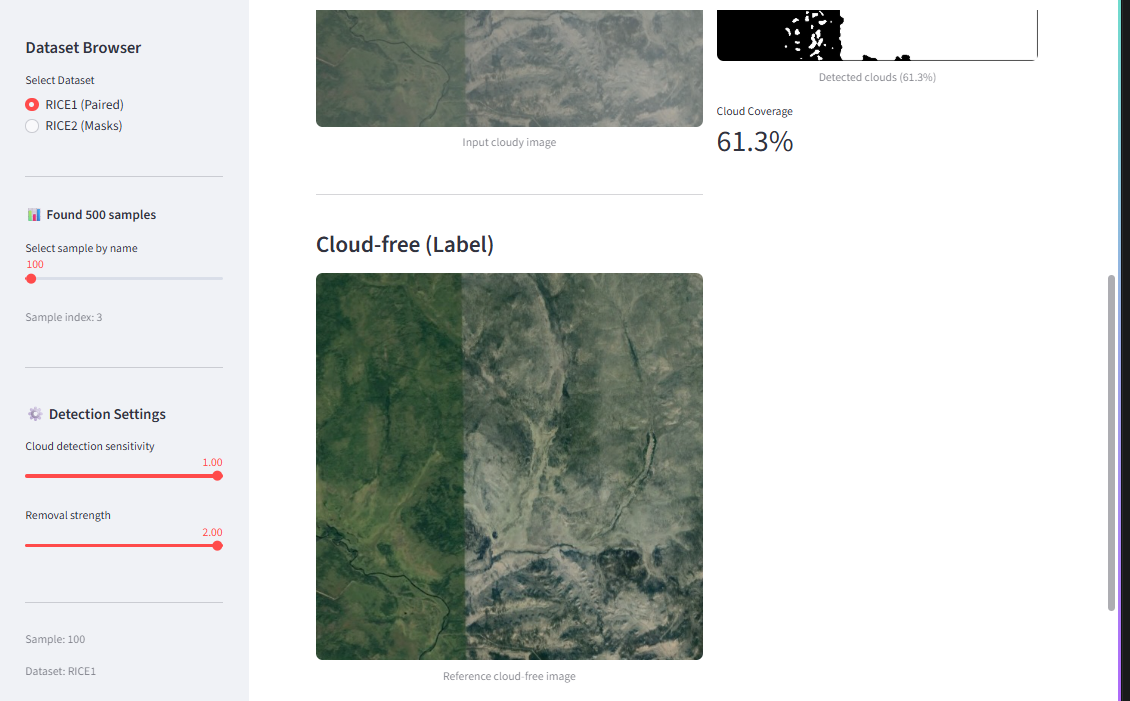
\includegraphics[width=\linewidth]{figures/rice1_provided_cloudfree.png}
  \caption{RICE1 cloud-free label screen}
\end{subfigure}

\vspace{0.3cm}

\begin{subfigure}{0.48\textwidth}
  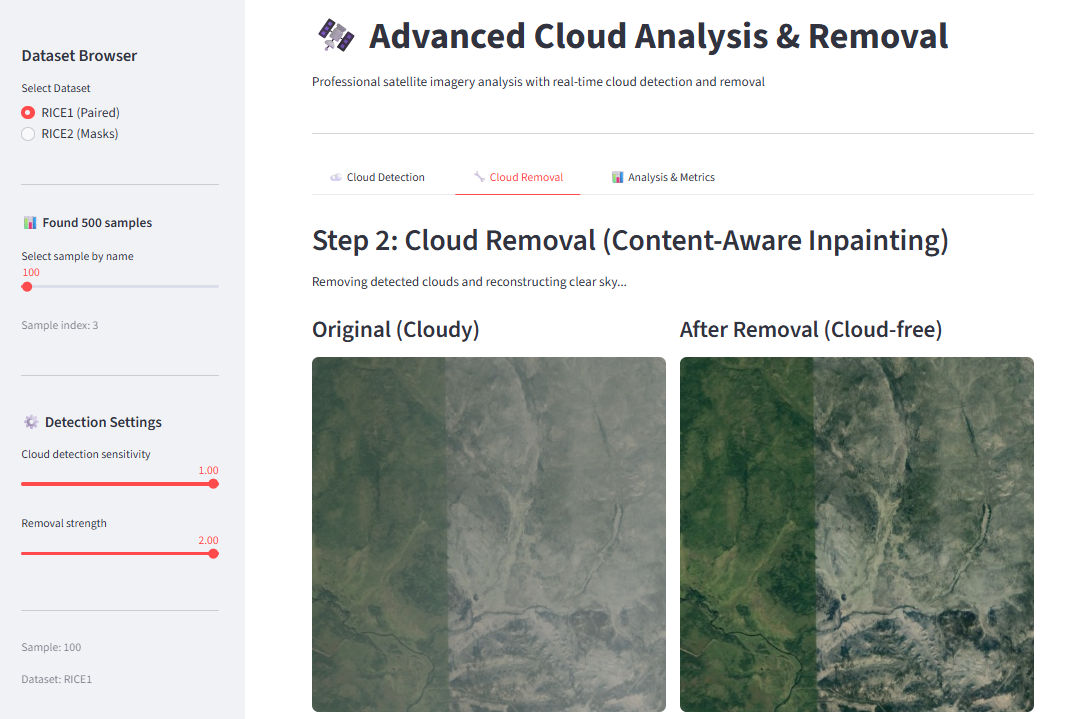
\includegraphics[width=\linewidth]{figures/rice1_provided_removal.png}
  \caption{RICE1 cloud-removal screen}
\end{subfigure}\hfill
\begin{subfigure}{0.48\textwidth}
  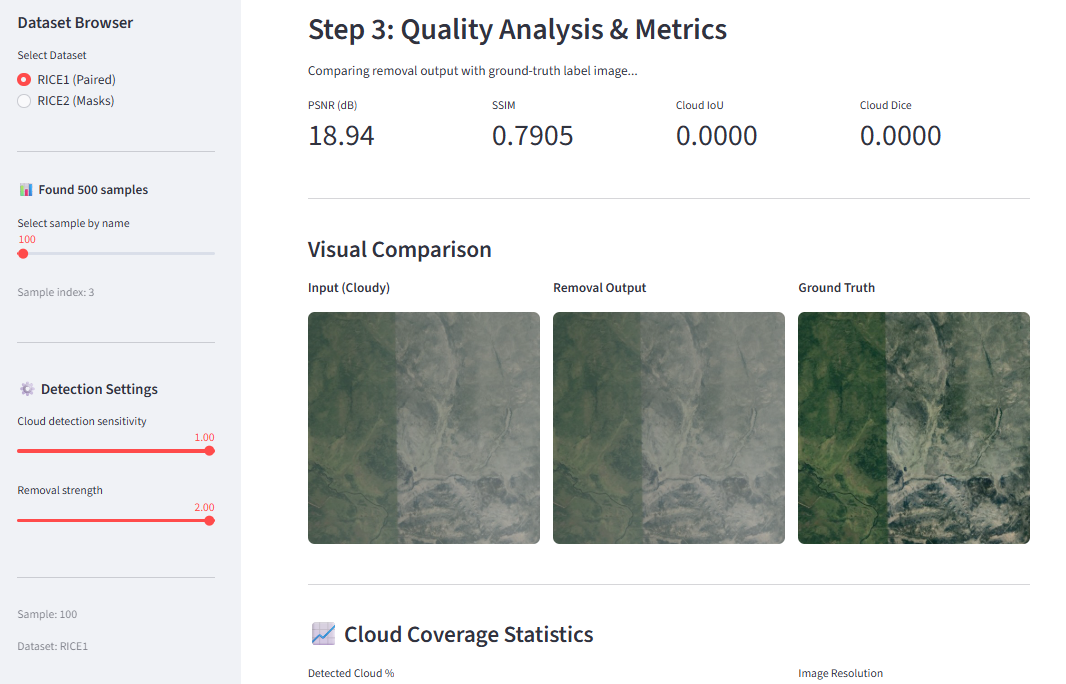
\includegraphics[width=\linewidth]{figures/rice1_provided_downloads_full.png}
  \caption{RICE1 download results screen}
\end{subfigure}
\caption{RICE1 sample 4: user-provided screenshot sequence}
\end{figure}

\begin{figure}[h]
\centering
\begin{subfigure}{0.48\textwidth}
  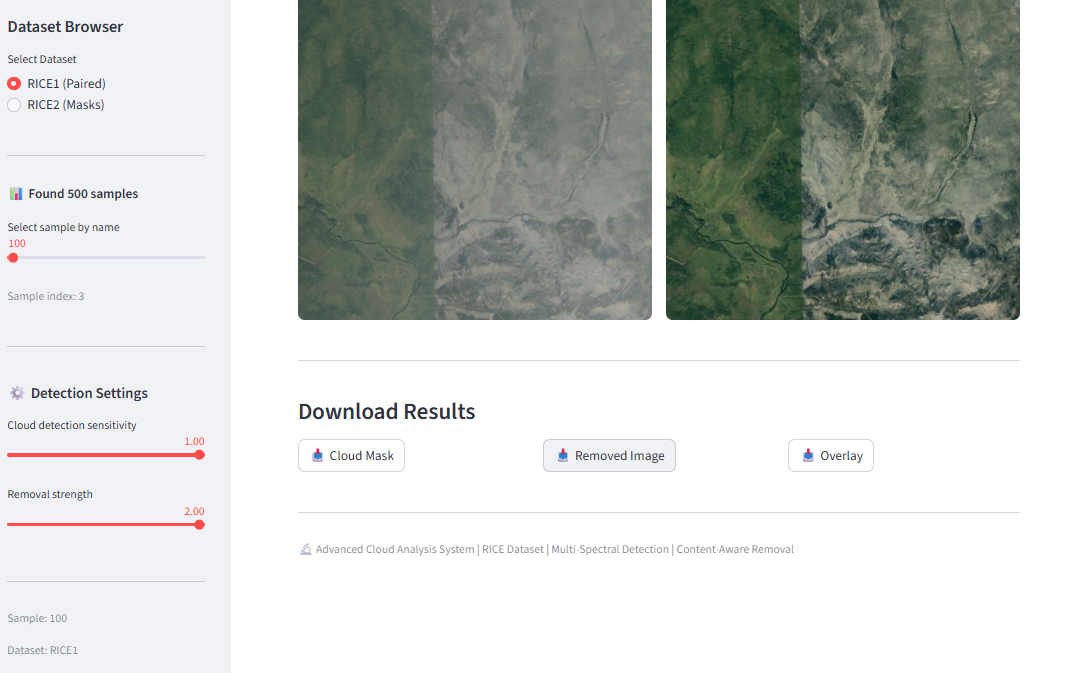
\includegraphics[width=\linewidth]{figures/rice1_provided_removal_close.png}
  \caption{RICE1 removal close-up}
\end{subfigure}\hfill
\begin{subfigure}{0.48\textwidth}
  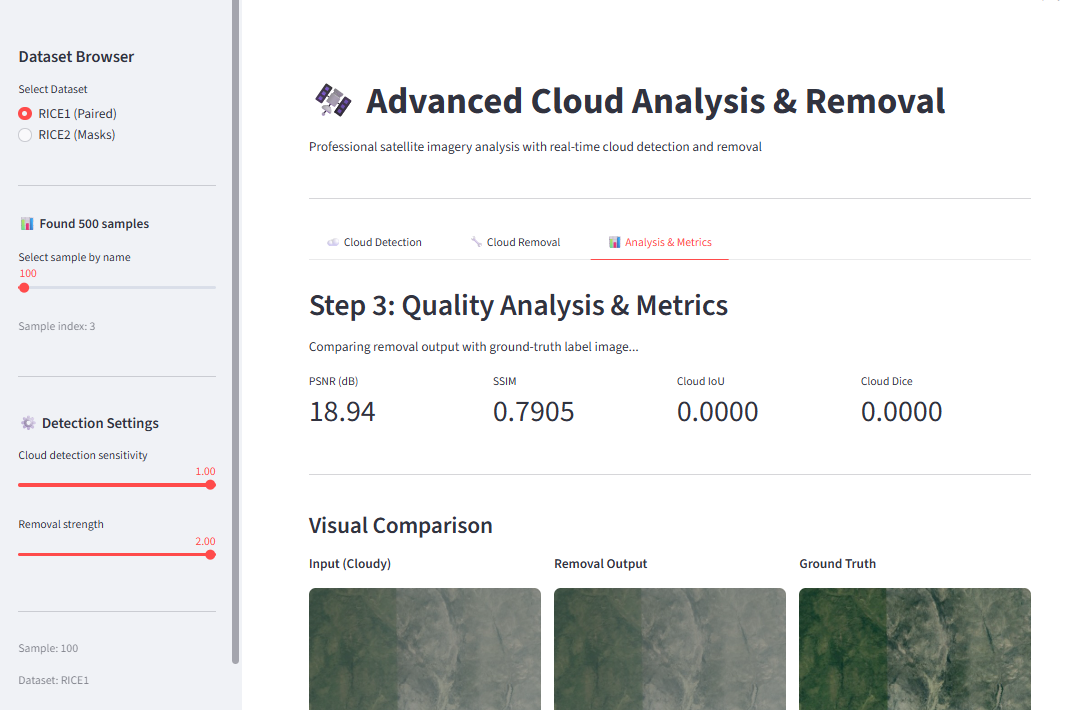
\includegraphics[width=\linewidth]{figures/rice1_provided_downloads_top.png}
  \caption{RICE1 download top section}
\end{subfigure}

\vspace{0.3cm}

\begin{subfigure}{0.48\textwidth}
  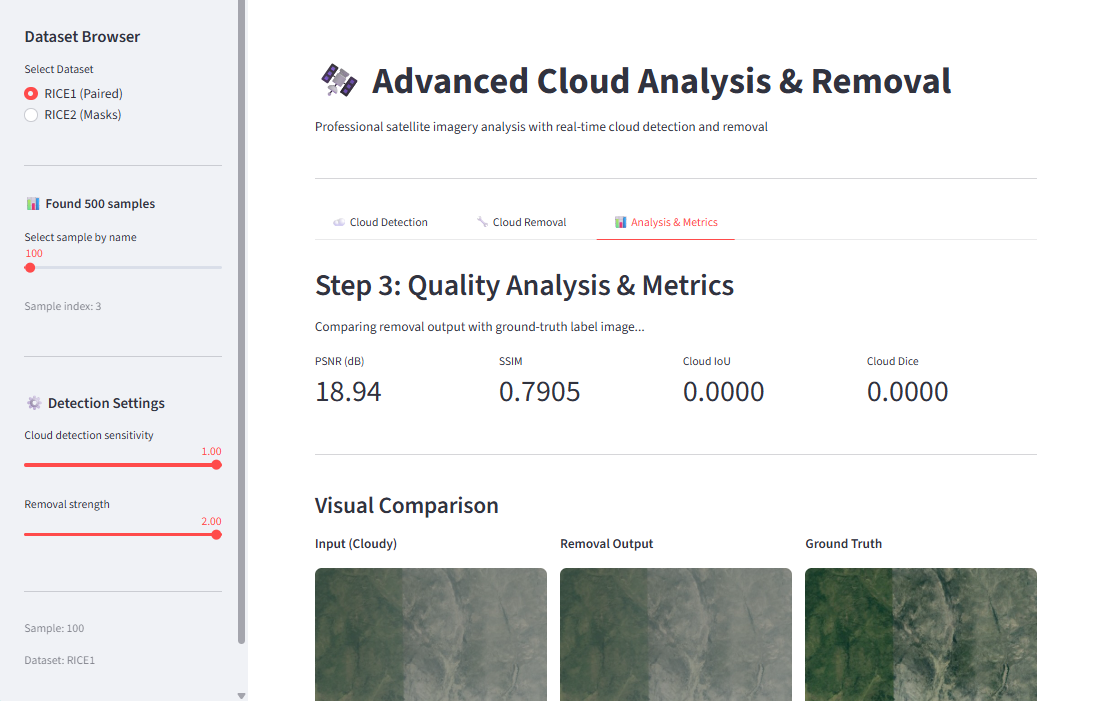
\includegraphics[width=\linewidth]{figures/rice1_provided_downloads_bottom.png}
  \caption{RICE1 download bottom section}
\end{subfigure}\hfill
\begin{subfigure}{0.48\textwidth}
  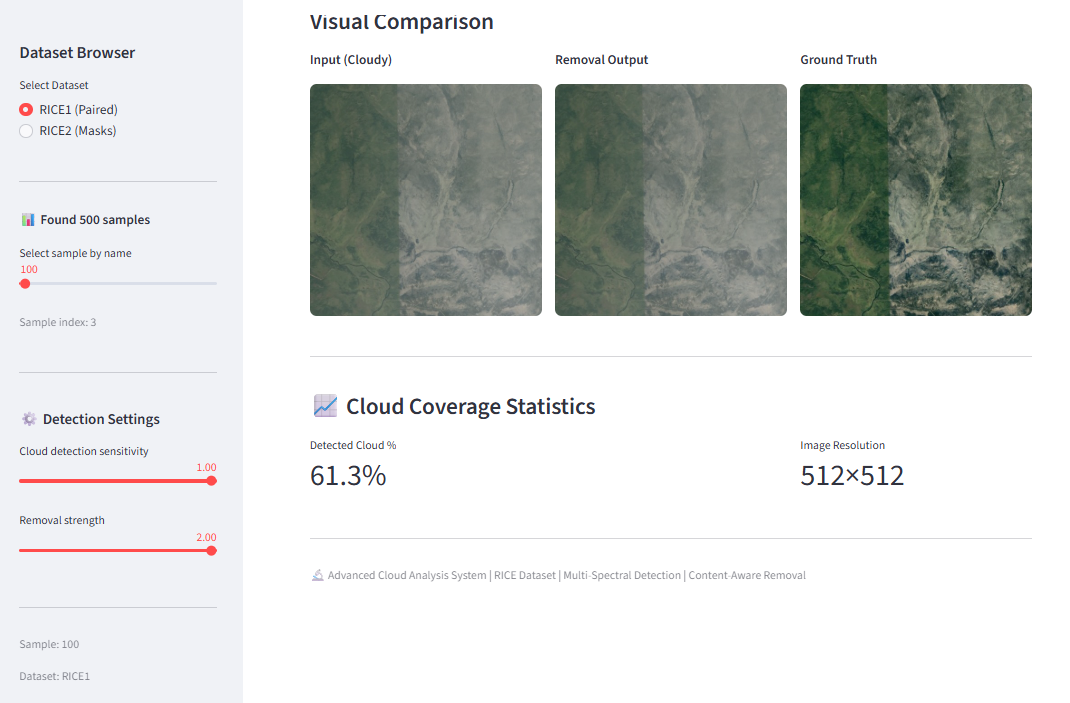
\includegraphics[width=\linewidth]{figures/rice1_provided_analysis_full.png}
  \caption{RICE1 analysis screen with metrics}
\end{subfigure}
\caption{RICE1 sample 4: additional provided screenshots}
\end{figure}

\section{Outputs and results}
The app produces the following visible outputs:
\begin{itemize}
  \item detected cloud mask,
  \item cloud coverage percentage,
  \item cloud-free reference display for RICE1 and RICE2,
  \item after-removal view,
  \item PSNR, SSIM, IoU, and Dice metrics,
  \item downloadable PNG artifacts for the mask, removed image, and overlay.
\end{itemize}

On the current RICE1 screenshot set, the Analysis and Metrics tab shows a visual comparison of input cloudy image, removal output, and ground truth, along with image quality metrics.

\section{How to reproduce}
\begin{verbatim}
python -m venv .venv
.\.venv\Scripts\Activate.ps1
pip install -r requirements.txt
streamlit run ui/app.py
\end{verbatim}

To compile the report on Windows, run the helper batch file in \verb|report/| or use \verb|pdflatex| directly.

\section{What is not used in the current program train}
The following parts are present in the repository but are not part of the current running Streamlit pipeline or training smoke test:
\begin{itemize}
  \item \verb|models/classification/| - empty scaffold.
  \item \verb|models/removal/| - empty scaffold.
  \item \verb|explainability/captum_utils.py| - not connected to the current UI flow.
  \item \verb|ui/model_manager.py| - helper class available, but the current app uses the advanced heuristic pipeline instead of this manager.
  \item \verb|configs/default.yaml| - configuration file exists, but the present app does not load it directly.
  \item \verb|notebooks/| - exploratory work, not part of runtime.
  \item \verb|data/raw/| and \verb|data/processed/| - storage folders, not directly consumed by the current execution path.
\end{itemize}

\section{Conclusion}
The project combines a practical cloud-detection and cloud-removal UI with a reproducible dataset loader, segmentation training code, and downloadable outputs. The report now includes the actual UI screenshots, the full folder map, the active libraries and models, and a final note about repository items that are not used in the current program train.

\end{document}
